% Synchronized to r30045

\marklabel{sec:opt-cpanel}
{
\section {OPT\_CPANEL}
}

\subsection{Introduction}

This packet allows to connect up to four buttons to the serial port of the fli4l router.
Pressing one key triggers a system command, for example halt or reboot. The buttons can be 
freely configured. There are 14 variations possible (theoretically there are 15 possibilities, but 
with the 15th the hardware does not work). 

The power / status LED (LED2) glows green as soon as the circuit is ready. During 
processing a command, the LED blinks. 
LED1 can be freely configured (further details below).


\subsection{Key Mapping}

The keys match the following values:

\begin{itemize}
    \item Key 1 = 1
    \item Key 2 = 2
    \item Key 3 = 4
    \item Key 4 = 8
\end{itemize}

If multiple keys are pressed simultaneously the values are added together. This gives 
the function number for the command.

The commands to be executed are inserted into these lines::
\var{OPT\_CPANEL\_FUNKTION1}='command'
Some commands require the full pathname.

Some Examples:
\begin{verbatim}

fli4lctrl dial pppoe		Dial in into DSL
fli4lctrl hangup pppoe		Drop the DSL connection 
isdnctrl dial ippp0		Dial in into ISDN
isdnctrl hangup ippp0		Drop the ISDN connection
/sbin/reboot			Reboot router
/sbin/halt			Shutdown router

\end{verbatim}

\subsection{Configuring The Status Display}

There are four possibilities to map the status LED.

DSL: 

Determine and show only the DSL status.

ISDN: 

Determine and show the ISDN status. All circuits are sumarized. If at least
one ISDN circuit is online, the LED1 glows.

DSLISDN:

Determine and show both DSL and ISDN status of all circuits.

SCRIPT:

Establish an own query. Take care of the following:
\begin{itemize}
    \item Insert only the commands.
    \item \#!/bin/sh will be added automatically.
    \item To light LED1 'on' has to be written into /var/run/cpanel.status (without ' ').
    \item To clear LED1 'off' has to be written into /var/run/cpanel.status 
    \item To let the LED blink, 'blink' has to be written into /var/run/cpanel.status. 
          The LED1 will blink until it is set to 'off' or 'on'.
\end{itemize}

Example:

This entry queries the DSL status:
\begin{verbatim}
echo off > /var/run/cpanel.status
fli4lctrl status | grep online >/dev/null && echo on > /var/run/cpanel.status
\end{verbatim}
Hint:
Use only if you know what you do. A faulty entry can cause that cpanel doesn't start
at all or does not work as expected.

\subsection{Troubleshooting}
\subsubsection{Hardware}

If it doesn't work instantly, check your circuit. Take care of the right pins of your 
PC plug. If your router still has a 25 pin serial port the pinout is different to the one in 
the circuit drawing!
If there is no error in your circuit, check the cable from your mainboard to the plug at the 
case. As there is no standard by the mainboard manufacturers there are different cables available.
In doubt, check your mainboard user guide.

\subsubsection{Software}

First check if cpanel starts at boottime. Near the end of the boot should appear a message. 
You can look at the process list by typing 'ps ax' at the console. If there is no cpanel in 
the list, you probably configured in config/cpanel.txt the item \var{OPT\_CPANEL} to 'no'. 
The graphics card could be a further source of errors. If you don't have a graphics card
in your router, the first serial port (COM1) is used for the console. If so, you have to
configure \var{CPANEL\_PORT}='/dev/ttyS0' to '/dev/ttyS1'. Of course the circuit has to be
connected to COM2.

\subsection{Miscellaneous}

  \begin{figure}[htbp]
    \centering
    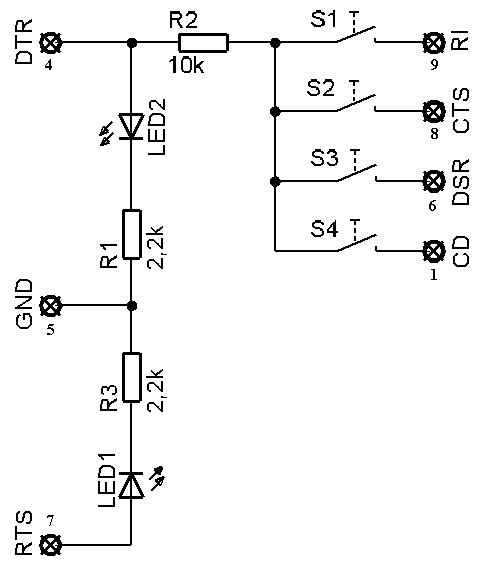
\includegraphics[width=485pt]{schematic}
    \caption{Wiring Plan}
    \label{fig:schaltplan}
  \end{figure}


\wichtig{There is no liability of any kind for any damages!}

Any problems, stories of success and suggestions for improvement may be posted to the newsgroup slpine.fli4l.opt.

Thank you for reading this documentation. Have fun with cpanel!
